\section{Nombre: Caja} \label{obs.caja}
\subsection{Descripción}
Una caja de madera. El jugador al tocar tendrá una característica rígida. El jugador no podrá moverla, puede pararse sobre ella. No ocasiona ningún efecto adicional al tocarla.
\subsection{Esquema}
Ver figura \ref{fig:caja}.
\begin{figure}
	\centering
	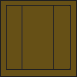
\includegraphics[height=0.2 \textheight]{Imagenes/caja}
	\caption{Caja de madera.}
	\label{fig:caja}
\end{figure}